\newsec{Considerazioni su $ V_{H}(i_{p}) $}

\subsection{Incompatibilità delle quote con $ 0 $}

Nelle regressioni lineari sulle curve $ V_H(i_p) $ (cioè tensione di Hall al variare della corrente nella sonda, per valori di campo magnetico $ B $ fissato), abbiamo trovato che le maggior parte delle quote non sono compatibili con $ 0 $.
Solo per le curve corrispondenti a valori di campo magnetico negativi c'è compatibilità, che addirittura migliora all'aumentare (in valore assoluto) del campo.

In realtà, però, i valori sperimentali di $ V_H(0) $ sono sempre compatibili con $ 0 $.
Il fatto che le regressioni ``preferiscano'' avere $ q \neq 0 $ è dovuto a degli effetti che si manifestano solo per valori di corrente $ i_p \neq 0 $.

A conferma di questo, possiamo studiare il caso della curva $ V_H(i_p) $ per $ B=0 $, cioè quella che abbiamo usato per caratterizzare la caduta di potenziale ohmica dovuta al disallineamento delle piastre.
Possiamo provare a usare come modello per la regressione una quota con $ q=0 $: il fit è accettabile (con un $ p $-value minore rispetto al modello con la quota ovviamente)\footnote{Precisamente otteniamo $ m = (0.0542 \pm 0.0002) \unit{mV/mA} $ con $ p = 0.998 $.} e la stima che otteniamo per il coefficiente angolare è compatibile con quella ricavata dal modello lineare completo (che è $ m_\text{all} = (0.0542 \pm 0.0002) \unit{mV/mA} $).

La compatibilità tra le stime dei coefficienti angolari supporta la bontà della stima che abbiamo dato di $ R_H $: se correggendo per la traslazione i coefficienti angolari non vengono modificati, allora essa non ne risente.

Resta anche da spiegare perché nella presa dati a $ B=0 $ il segno della quota sia positivo, contrariamente a tutte le altre curve.

\begin{table}
\centering \small
\begin{tabular}{cc|cc|ccc}
$B$ & $\delta B$ & $q$ & $\delta q$ & $q_\text{corr}$ & $\delta q_\text{corr}$ & $Z$ \\
\hline
48 & 9 & -0.009 & 0.002 & -0.006 & 0.002 & 2.629 \\
101 & 10 & -0.008 & 0.003 & -0.005 & 0.003 & 1.786\\
147 & 10 & -0.009 & 0.003 & -0.006 & 0.003 & 1.867 \\
193 & 10 & -0.008 & 0.003 & -0.005 & 0.003 & 1.368 \\
240 & 11 & -0.008 & 0.003 & -0.004 & 0.003 & 1.289  \\
-48 & 9 & -0.0027 & 0.0015 & 0.0005 & 0.0018 & -0.283\\
-98 & 10 & -0.003 & 0.002 & 0.000 & 0.003 & 0.036\\
-145 & 10 & -0.001 & 0.003 & 0.002 & 0.003 & -0.793\\
-194 & 10 & 0.000 & 0.003 & 0.003 & 0.003 & -1.067\\
-238 & 11 & 0.000 & 0.003 & 0.003 & 0.003 & -0.978
\end{tabular}
\caption{Valori delle quote (in $ \unit{mV} $) corrispondenti ai fit di $ V_H(i_p) $ per i valori di $ B $ (in $ \unit{mT} $) prima e dopo la correzione descritta nella sezione (B.2). Riportiamo anche i valori dei test Z di compatibilità tra le quote corrette e $ 0 $: sulle quote corrette abbiamo propagato gli errori considerando anche il contributo dato dall'incertezza sulla quota del contributo del disallineamento.: sulle quote corrette abbiamo propagato gli errori considerando anche il contributo dato dall'incertezza sulla quota della caratteristica del contributo del disallineamento.}
\label{tab:qcorr}
\end{table}


\subsection{Possibili spiegazioni}

Crediamo che ci siano due effetti distinti in gioco:
\begin{enumerate}
\item un contributo additivo alla caduta di potenziale ohmica dovuta al disallineamento delle piastre,
\item un contributo additivo alle caratteristiche $ V_H(i_p) $ antisimmetrico al segno di $ B $.
\end{enumerate}

La fonte del primo contributo potrebbe essere attribuita a un'asimmetria geometrica nella sonda di Hall.
Prendendo di nuovo come esempio il caso della curva con $ B=0 $ (per cui non si manifesta nemmeno l'altro fenomeno), possiamo fare delle regressioni per $ i_p \geq 0 $ e $ i_p \leq 0 $ separatamente.
Troviamo che entrambe le curve vengono approssimate in modo accettabile da delle rette con quota nulla:\footnote{Cioè con quote che sono compatibili con $ 0 $.}:
\begin{equation}
m_\text{pos} = (0.0551 \pm 0.0005) \unit{mV / mA} \qquad q_\text{pos} = (-0.001 \pm 0.002) \unit{mV}
\end{equation}
con $ p = 1.00 $, e:
\begin{equation}
m_\text{neg} = (0.0537 \pm 0.0005) \unit{mV / mA} \qquad q_\text{neg} = (0.001 \pm 0.002) \unit{mV}
\end{equation}
con $ p = 0.998 $, quindi nel primo caso $ m_\text{pos} > m_\text{all} $, mentre nel secondo $ m_\text{neg} < m_\text{all} $ (ricordiamo che $ m_\text{all} = (0.0542 \pm 0.0002) \unit{mV/mA} $).

Addirittura $ m_\text{neg} - m_\text{all} $ e $ m_\text{all} - m_\text{pos} $ sono compatibili tra loro.
Facendo fluire la corrente nei due versi, stiamo misurando una tensione di Hall extra pari a:
\begin{equation}
V_{H,\text{extra}} = k \cdot \abs{i_p}
\end{equation}
dove $ k \simeq \abs{m_\text{neg} - m_\text{all}} $, che si somma  alla caduta di potenziale ohmica $ V_{H} = m i_p $.

Diciamo che il contributo è dovuto a un'asimmetria, perché nelle curve relative a $ B \neq 0 $ abbiamo misurato dei contributi extra alla tensione di Hall $ V_{H,\text{extra}} = - k \abs{i_p} $ ($k>0$).\footnote{Se $ k>0 $ porta ad avere delle quote positive, allora $ k<0 $ le sposta verso valori negativi.}
La nostra ipotesi è che il segno di $ k $ dipenda dall'orientazione della sonda di Hall: per la presa dati con $ B=0 $ abbiamo assegnato il verso positivo alla corrente che fluisce dalla connessione $ \alpha $ verso quella $ \beta $, mentre per quelle con $ B \neq 0 $ abbiamo considerato positiva la corrente che si muove da $ \beta $ verso $ \alpha $.\footnote{In un caso e nell'altro abbiamo applicato il campo magnetico necessario a misurare la tensione di Hall in maniera concorde, controllando la direzione in cui abbiamo applicato $ B $, e quella in cui abbiamo misurato $ V_H $.}

Il fatto che il comportamento misurato sia pari in $ i_p $ suggerisce che il fenomeno a valori di $ i_p $ più grandi potrebbe essere proporzionale a $ i_p^2 $, e quindi dipendere da effetti termici (la potenza dissipata sulla sonda va con $ i_p^2 $).

Tenendo in considerazione la differenza di segno di $ k $, per correggere questo fenomeno è sufficiente sommare $ q_{B=0} \simeq 0.0035 \unit{mV} $ alle quote in \cref{fig:intercepts}:\footnote{Ci si può convincere facilmente che il contributo $ k\abs{i_p} $ non modifica il coefficiente angolare ottenuto dalle regressioni.} troviamo che i due gruppi di quote (distinti dal segno di $ B $) si raccolgono intorno a $ q \simeq \pm 0.004 \unit{mV} $.

\begin{figure}
\centering
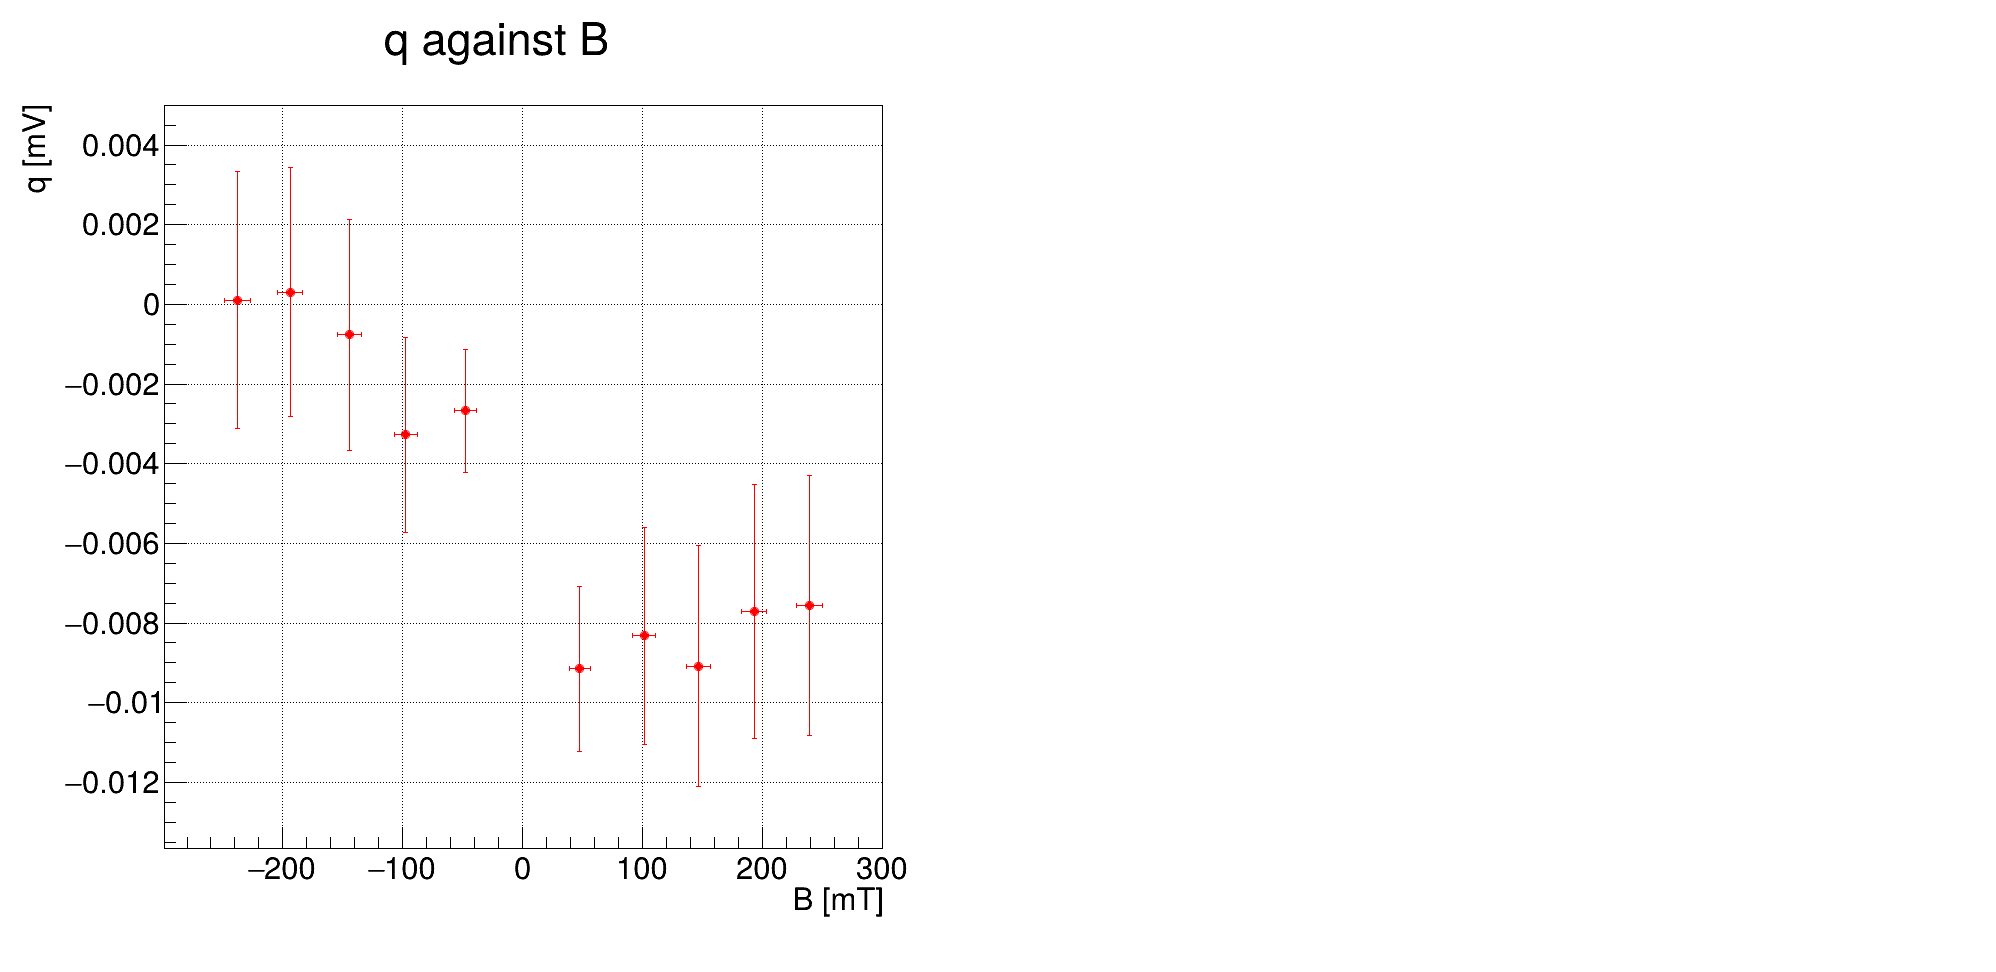
\includegraphics[width=0.85\textwidth]{./figs/intercepts.png}
\caption{Quote ($q$ in \unit{mV}, riportate in \cref{tab:qcorr}) ricavate dalle regressioni (con il modello completo, sul range completo) per ogni valore di $ B \neq 0 $ (in $ \unit{mT} $). Si vede come i contributi per $ B>0 $ e $ B<0 $ popolano due regioni ben distinte del piano.}
\label{fig:intercepts}
\end{figure}

Correggendo per questo contributo (sommando la quota della curva $ B=0 $ a quella di tutte le altre), le quote di tutte le regressioni si avvicinano allo $ 0 $ diventando compatibili.
Comunque, si osserva che tutte le quote si distribuiscono asimmetricamente con il segno di $ B $, anche dopo la correzione.
Avendo a disposizione così pochi dati è difficile caratterizzare un fenomeno che possa spiegare questa asimmetria: potrebbe avere nuovamente una natura geometrica, come potrebbe dipende anche da dei bias strumentali.
